\documentclass[12pt, a4paper, oneside]{ctexart}
\usepackage{amsmath,amsthm,amssymb,graphicx}
\usepackage[ bookmarks=true,colorlinks,citecolor=blue,linkcolor=black ]{hyperref}
\usepackage{booktabs, tabularx}
\usepackage{float}

\usepackage[utf8]{inputenc}
\usepackage{pgfplots}
\pgfplotsset{compat=1.18}
\usepackage{geometry}
%注释用的是百分号
\title{\textbf{大作业报告}}
\author{Xuankun Yang}
\date{2025年6月7日}

\begin{document}

\maketitle
\tableofcontents

\section{数据预处理}

\subsection{表格数据预处理}
在表格数据预处理部分,我按照下面的步骤来进行:
\begin{enumerate}
    \item 将五张表格中的数据通过\texttt{Pandas}读取得到,然后根据读取的年份排序。
    通过观察每一张表中的\emph{Survey Date},不难发现在每一张表格内部日期是升序排列的,所以我这里只是简单地按年份排序。
    \item 
    {
        根据表格中的列名,分出来四类特征,并对齐进行了不同的操作。
        \begin{itemize}
            \item 目标特征:\emph{'Number of nights in CITY'}和\emph{'Purpose of visit to CITY'},这是我们需要预测的变量,对缺省值只分别进行简单的中位数和众数填充。
            \item 数值型特征:例如\emph{'Age'}、\emph{'Total expenditures'}等,对其的处理在后面的不同处理方法中讨论。
            \item 类别型特征:例如\emph{'Nationality'}、\emph{'Gender'}等,我对这些没有做独热编码的特征进行了独热编码,防止模型将其视作数值型特征。
            \item 已经编码过的类别特征:例如\emph{'Companion\_1', 'Companion\_2'}、\emph{'Transportation 01', 'Transportation 02'}等,
            在这些特征中可能存在多列都是1的情况,我将其视为多项选择,不做处理。
            \item 层次型特征:例如\emph{'Satisfaction level by item 01', 'Satisfaction level by item 02'}等,通过数据特征说明表得知,
            虽然每一列的选项数是固定的,但是不同选项之间是存在层级关系的,对此我使用\texttt{OrdinalEncoder()}工具进行编码。
        \end{itemize}
    }
    \item 不难发现,表格中存在许多缺省值,对于这些缺省值的处理,在我不同的数据处理方法中采用了不同的方式,下面进行介绍。
    
\end{enumerate}

我尝试了多种不同的方法,然后使用最简单的线性模型
\texttt{Linear Regression}进行回归任务并比较不同预处理方法下的模型性能。

\subsection{方法一}
这是最朴素的方法,关键的处理步骤如下:
\begin{itemize}
    \item 对连续型特征,缺省值采用中位数进行填充
    \item 对于类别型特征,缺省值采用众数进行填充,之后进行独热编码
    \item 对于\emph{Nan}值使用平均数替换
    \item 根据\emph{'Number of nights in CITY'}和\emph{'Total expenditures'}计算得到新特征,即每天的平均消费
\end{itemize}

这样处理之后得到的数据维度为(72370, 386)。

通过方法一得到一组预处理好的数据,进行两组实验,一组做归一化,一组不做归一化,分别使用\texttt{Linear Regression}进行回归任务,
并做出每一折中\textbf{残差绝对值}关于数据点下标的图,发现两组中均出现残差绝对值特别大的点,也正是这些点导致最终的\emph{MSE}和\emph{$R^2$}系数表现很差。
\begin{figure}[H]
    \centering
    \includegraphics[width=0.8\textwidth]{Figs/abs_residual_scaled.png}
    \caption{归一化组的残差绝对值}
    \label{fig: abs_residual_scaled}
\end{figure}

\begin{figure}[H]
    \centering
    \includegraphics[width=0.8\textwidth]{Figs/abs_residual_unscaled.png}
    \caption{未归一化组的残差绝对值}
\end{figure}
于是,我又进行了新方法的尝试。

\subsection{方法二}
下面是关键的处理步骤:
\begin{itemize}
    \item 设置一个缺省阈值$p$,当某一个特征缺省样本比例大于$p$时进行丢弃
    \item 对于每一个数值型特征,求出其均值$\mu$与标准差$\sigma$,设置一个标准差倍数阈值$k$,直接丢弃该特征不在区间$\left[\mu - \sigma, \mu + \sigma\right]$的数据点
    \item 对剩下的特征和样本点进行同样的缺省值填充
    \item 删除重复数据点
    \item 对于\emph{Nan}值使用众数替换
    \item 不加入每天的平均消费这一特征
\end{itemize}

同样的,设置$p=0.2, k=3$,这样得到的数据维度为(71214, 226)。

对于使用方法二预处理好的数据,进行两组实验,一组做归一化,一组不做归一化,分别使用\texttt{Linear Regression}进行回归任务,
同样做出每一折中残差绝对值关于数据点下标的图。

\begin{figure}[H]
    \centering
    \includegraphics[width=0.8\textwidth]{Figs/abs_residual_Scaled\_augmented.png}
    \caption{归一化组的残差绝对值}
\end{figure}

\begin{figure}[H]
    \centering
    \includegraphics[width=0.8\textwidth]{Figs/abs_residual_unScaled\_augmented.png}
    \caption{未归一化组的残差绝对值}
\end{figure}
可以看出,进行这种数据处理方法之后,做归一化的组的残差仍很大,而对于不做归一化处理的组有较好的增益。

之后我又在思考,这具体是什么原因,我觉得可能还是因为数据中的极端值以及$k$和$q$的值设置得不恰当导致的,于是提出了更为朴素的新方法。
\subsection{方法三}

方法三是基于方法一进行改进的,改进点如下:
\begin{itemize}
    \item 由方法一得到数据,使用\texttt{Linear Regression},得到残差,做出残差绝对值图,设置阈值$t$,当残差绝对值大于$t$时,选择将该数据点丢弃
\end{itemize}

由图\ref{fig: abs_residual_scaled},看出使用归一化后,残差的波动较大,不好设置阈值,因此,设置阈值只针对不做归一化的组。

设置阈值$t=5000$,得到的数据维度为(72361, 386),可以看出相较于方法一仅删去了9个数据点,同样做出残差绝对值图。

\begin{figure}[H]
    \centering
    \includegraphics[width=0.8\textwidth]{Figs/abs_residual_unScaled\_after_unscaled.png}
    \caption{归一化组的残差绝对值}
\end{figure}

\begin{figure}[H]
    \centering
    \includegraphics[width=0.8\textwidth]{Figs/abs_residual_unScaled\_after_unscaled.png}
    \caption{未归一化组的残差绝对值}
\end{figure}

同样的,使用这种方法发现,对于做归一化的组,尽管已经丢弃了一些极端点,但是会出现新的残差较大的点。
但是对于不做归一化的组,丢掉一些极端点之后整体的残差绝对值会小很多。在后面的实验中,我主要使用方法二和方法三,并会做一些对比。

\section{特征工程}
在特征工程这一部分中,我主要进行了以下几种特征学习的方法:
\begin{itemize}
    \item 主成分分析(PCA)
    \item 特征选择
    \item 线性判别分析(LDA)
\end{itemize}

此外,我还探究了归一化对模型以及特征学习的影响,因此是否做归一化将与这些特征学习技术进行组合来进行实验。

与此同时,我对数据预处理方法进行了交叉组合后进行了大量实验,具体效果会视具体模型进行讨论。

\subsection{主成分分析}
在本次任务中,为了探究使用 PCA 降维之后的维度对于实验结果的影响,我设置了三种维度,分别为 50,100,200。

\subsection{特征选择}
同样的,对于特征选择之后的维度,我设置了三个,50,100,200。

对于回归任务,选用评分函数\texttt{f\_regression},对于分类任务,选用默认评分函数\texttt{f\_classif}。

\subsection{线性判别分析}
该方法仅针对分类任务。
由于我们类别数$C$只有4,为保证降维之后信息的完整,选择降维后的维度为$C - 1$,即降至3维。

\subsection{交叉验证}
进行完数据预处理以及特征学习之后,使用\texttt{sklearn.model\_selection.TimeSeriesSplit(n\_splits = 5)}进行时间序列的划分,
保证模型学习的数据在待预测的数据之前采样。

\section{回归任务}
\subsection{模型以及指标选择}
\begin{itemize}
    \item 
    {
        在回归任务中,我主要探究了以下几种模型:
\begin{itemize}
    \item 线性模型:\texttt{Linear Regression}
    \item 带正则化的线性模型:\texttt{Ridge}、\texttt{Lasso}
    \item 非线性模型:\texttt{Decision Tree}、\texttt{Polynomial Regression}以及使用\texttt{'rbf'}核函数的\texttt{SVR}
    \item 集成学习:\texttt{Random Forest}、\texttt{Bagging}、\texttt{Stacking}
\end{itemize}
    }
    \item 
    {
        在该任务中,我选用了\emph{MSE}、\emph{MAE}以及\emph{$R^2$}系数这三种指标。
\begin{itemize}
    \item \emph{Mean Squared Error (MSE)}:
    \[
    \text{MSE} = \frac{1}{n} \sum_{i=1}^{n} \left( y_i - \hat{y}_i \right)^2
    \]

    \item \emph{Mean Absolute Error (MAE)}:
    \[
    \text{MAE} = \frac{1}{n} \sum_{i=1}^{n} \mid y_i - \hat{y}_i \mid
    \]

    \item \emph{Coefficient of Determination ($R^2$)}:
    \[
    R^2 = 1 - \frac{\sum_{i=1}^{n} \left( y_i - \hat{y}_i \right)^2}{\sum_{i=1}^{n} \left( y_i - \bar{y}_i \right)^2} = 1 - \frac{\text{MSE}}{\text{Var}(y)}
    \]
\end{itemize}

        不难看出,测试数据方差一定时,\emph{MSE}和\emph{$R^2$}系数之间有较强的联系。
    }
\end{itemize}

\subsection{线性模型}
\subsubsection{\texttt{Linear Regression}}
对于简单的线性回归,我做了丰富的实验,得到下表\ref{tab: Linear Regression}中的数据,其中**表示该设置下模型效果很差,不做展示。

\begin{table}[H]
    \centering
    \small % Reduce font size to fit content better
    \setlength{\tabcolsep}{3.5pt} % Adjust column padding for tighter fit
   \resizebox{\linewidth}{!}{
    \begin{tabular}{|l|c|c|c|c|c|c|}
    \hline
    \textbf{Feature Set} & \multicolumn{3}{c|}{\textbf{方法二}} & \multicolumn{3}{c|}{\textbf{方法三}} \\ \cline{2-7}
     & \textbf{Avg MSE} & \textbf{Avg MAE} & \textbf{Avg $R^2$} & \textbf{Avg MSE} & \textbf{Avg MAE} & \textbf{Avg $R^2$} \\ \hline
    Original & 117.5765 & 3.2744 & 0.0306 & 403.5197 & 7.2216 & -0.0218 \\ \hline
    PCA\_50 & 117.1318 & 3.2199 & 0.0350 & 21559.1233 & 17.9094 & -59.1558 \\ 
    PCA\_100 & 18086.2861 & 31.8863 & -113.8824 & 28580.4110 & 20.1809 & -78.2481 \\ 
    PCA\_200 & ** & ** & ** & ** & ** & ** \\ \hline
    Select50Best & 117.3058 & 3.2807 & 0.0287 & 364.1845 & 6.6408 & 0.0921 \\ 
    Select100Best & 117.1462 & 3.2598 & 0.0341 & 368.1107 & 6.7700 & 0.0793 \\ 
    Select200Best & 117.5202 & 3.2641 & 0.0311 & 385.5867 & 6.9961 & 0.0292 \\ \hline
    Scaled\_Original & ** & ** & ** & ** & ** & ** \\ \hline
    Scaled\_PCA\_50 & 117.1318 & 3.2199 & 0.0350 & 21559.1233 & 17.9094 & -59.1558 \\ 
    Scaled\_PCA\_100 & 18086.2861 & 31.8863 & -113.8824 & 28580.4110 & 20.1809 & -78.2481 \\ 
    Scaled\_PCA\_200 & ** & ** & ** & ** & ** & ** \\ \hline
    Scaled\_Select50Best & ** & ** & ** & \textbf{361.5178} & \textbf{6.6312} & \textbf{0.0978} \\ 
    Scaled\_Select100Best & ** & ** & ** & ** & ** & ** \\ 
    Scaled\_Select200Best & ** & ** & ** & ** & ** & ** \\ \hline
    \end{tabular}
    }
    \caption{Regression Metrics for Linear Regression}
    \label{tab: Linear Regression}
\end{table}
下面是取出最优参数设置的模型,对于每一折中的数据进行了可视化。

第一行为真实值与预测值的关系,第二行为残差绝对值和预测值之间的关系,第三行为残差分布。

\begin{figure}[H]
    \centering
    \includegraphics[width=0.8\textwidth]{Figs/reg_Linear_Regression.png}
    \caption{Linear Regression}
\end{figure}

下面我又取出了每一折中的性能指标。
\begin{figure}[H]
    \centering
    \includegraphics[width=0.8\textwidth]{Figs/reg_Linear_Regression_detailed.png}
    \caption{Linear Regression}
\end{figure}

此外,我也探索了正则化是否对模型性能有帮助,进行了下面带有正则化的线性模型的实验。
\subsubsection{\texttt{Ridge}}
在\texttt{Ridge}的训练过程中,我设置$\alpha$的取值为$\left[0.1, 1, 10, 100\right]$,
然后使用\texttt{GridSearchCV}进行参数搜索调优,得到下表中的结果。

\begin{table}[H]
    \centering
    \small % Reduce font size to fit content better
    \setlength{\tabcolsep}{3.5pt} % Adjust column padding for tighter fit
   \resizebox{\linewidth}{!}{
    \begin{tabular}{|l|c|c|c|c|c|c|}
    \hline
    \textbf{Feature Set} & \multicolumn{3}{c|}{\textbf{方法二}} & \multicolumn{3}{c|}{\textbf{方法三}} \\ \cline{2-7}
     & \textbf{Avg MSE} & \textbf{Avg MAE} & \textbf{Avg $R^2$} & \textbf{Avg MSE} & \textbf{Avg MAE} & \textbf{Avg $R^2$} \\ \hline
    Original & 117.0811 & 3.2453 & 0.0346 & 401.9578 & 7.1743 & -0.0177 \\ \hline
    PCA\_50 & 116.8604 & 3.2052 & 0.0368 & 14592.3453 & 15.4676 & -39.3786 \\ 
    PCA\_100 & 117.0597 & 3.2497 & 0.0348 & 462.4693 & 7.2489 & -0.1706 \\ 
    PCA\_200 & 117.0811 & 3.2453 & 0.0346 & 1855.9776 & 13.5501 & -4.0054 \\ \hline
    Select50Best & 117.0970 & 3.2699 & 0.0304 & \textbf{361.0409} & \textbf{6.6135} & \textbf{0.0985} \\ 
    Select100Best & 116.8291 & 3.2412 & 0.0366 & 370.3615 & 6.7160 & 0.0750 \\ 
    Select200Best & 117.0145 & 3.2334 & 0.0351 & 385.0843 & 6.9788 & 0.0303 \\ \hline
    Scaled\_Original & 117.4833 & 3.2828 & 0.0312 & 369.9627 & 7.1076 & 0.0734 \\ \hline
    Scaled\_PCA\_50 & 116.9829 & 3.2080 & 0.0360 & 488.5262 & 6.4774 & -0.2353 \\ 
    Scaled\_PCA\_100 & 117.3304 & 3.3319 & 0.0328 & 439.3663 & 7.1469 & -0.1053 \\ 
    Scaled\_PCA\_200 & 122.6151 & 3.2957 & -0.0123 & 424.7627 & 7.8393 & -0.0691 \\ \hline
    Scaled\_Select50Best & 117.2917 & 3.2787 & 0.0288 & 361.8132 & 6.6246 & 0.0985 \\ 
    Scaled\_Select100Best & 117.0739 & 3.2564 & 0.0346 & 362.9062 & 6.7454 & 0.0938 \\ 
    Scaled\_Select200Best & 117.4233 & 3.2598 & 0.0317 & 365.3024 & 6.9384 & 0.0866 \\ \hline
    \end{tabular}
    }
    \caption{Regression Metrics for Ridge}
\end{table}

同样的,取出最优参数设置的模型,下面是每一折中的性能表现。

\begin{figure}[H]
    \centering
    \includegraphics[width=0.8\textwidth]{Figs/reg_Ridge.png}
    \caption{Ridge}
\end{figure}

\begin{figure}[H]
    \centering
    \includegraphics[width=0.8\textwidth]{Figs/reg_Ridge_detailed.png}
    \caption{Ridge}
\end{figure}

\subsubsection{\texttt{Lasso}}
对于\texttt{Lasso},我选用了\texttt{LassoCV}来辅助找到最优的$\alpha$。
其中,最大迭代次数设置为10000,并使用默认的\texttt{n\_alpha}=100,得到下面的数据。

\begin{table}[H]
    \centering
    \small % Reduce font size to fit content better
    \setlength{\tabcolsep}{3.5pt} % Adjust column padding for tighter fit
   \resizebox{\linewidth}{!}{
    \begin{tabular}{|l|c|c|c|c|c|c|}
    \hline
    \textbf{Feature Set} & \multicolumn{3}{c|}{\textbf{方法二}} & \multicolumn{3}{c|}{\textbf{方法三}} \\ \cline{2-7}
     & \textbf{Avg MSE} & \textbf{Avg MAE} & \textbf{Avg $R^2$} & \textbf{Avg MSE} & \textbf{Avg MAE} & \textbf{Avg $R^2$} \\ \hline
    Original & 116.9855 & 3.1003 & 0.0361 & 582.9891 & 6.2168 & -0.4930 \\ \hline
    PCA\_50 & 117.0486 & 3.0802 & 0.0341 & 582.2179 & 6.2008 & -0.4924 \\ 
    PCA\_100 & 117.0486 & 3.0802 & 0.0341 & 582.2179 & 6.2008 & -0.4924 \\ 
    PCA\_200 & 117.0486 & 3.0802 & 0.0341 & 582.2179 & 6.2008 & -0.4924 \\ 
    Select50Best & 117.4585 & 3.1869 & 0.0278 & 501.6452 & 5.9179 & -0.2555 \\ \hline
    Select100Best & 116.9855 & 3.1003 & 0.0361 & 517.9338 & 5.9447 & -0.3027 \\ 
    Select200Best & 116.9855 & 3.1003 & 0.0361 & 543.6937 & 6.0199 & -0.3811 \\ 
    Scaled\_Original & 116.4797 & 3.1257 & 0.0378 & 342.0583 & 6.2306 & 0.1486 \\ \hline
    Scaled\_PCA\_50 & 116.3282 & 3.1457 & 0.0388 & 584.9696 & 6.4365 & -0.5145 \\ 
    Scaled\_PCA\_100 & 116.2892 & 3.1386 & 0.0390 & 434.4916 & 6.1971 & -0.0938 \\ 
    Scaled\_PCA\_200 & \textbf{116.2380} & \textbf{3.1301} & \textbf{0.0394} & 427.4175 & 6.7063 & -0.0802 \\ \hline
    Scaled\_Select50Best & 116.9840 & 3.1539 & 0.0318 & 351.7954 & 6.1054 & 0.1229 \\ 
    Scaled\_Select100Best & 116.4380 & 3.1296 & 0.0381 & 344.1170 & 6.1963 & 0.1433 \\ 
    Scaled\_Select200Best & 116.4768 & 3.1254 & 0.0378 & 342.2732 & 6.1990 & 0.1481 \\ \hline
    \end{tabular}
    }
    \caption{Regression Metrics for Lasso}
\end{table}

同样的,取出最优参数设置的模型,下面是每一折中的性能表现。

\begin{figure}[H]
    \centering
    \includegraphics[width=0.8\textwidth]{Figs/reg_Lasso.png}
    \caption{Lasso}
\end{figure}

\begin{figure}[H]
    \centering
    \includegraphics[width=0.8\textwidth]{Figs/reg_Lasso_detailed.png}
    \caption{Lasso}
\end{figure}

\subsection{非线性模型}

\subsubsection{\texttt{Polynomial Regression}}
在\texttt{Polynomial Regression}中,我对数值型特征(前11维)使用了\texttt{PolynomialFeatures(degree=2)}来进行二阶项的构造,
然后使用线性回归模型来进行拟合,得到下表中的结果。
\begin{table}[H]
    \centering
    \small % Reduce font size to fit content better
    \setlength{\tabcolsep}{3.5pt} % Adjust column padding for tighter fit
   \resizebox{\linewidth}{!}{
    \begin{tabular}{|l|c|c|c|c|c|c|}
    \hline
    \textbf{Feature Set} & \multicolumn{3}{c|}{\textbf{方法二}} & \multicolumn{3}{c|}{\textbf{方法三}} \\ \cline{2-7}
     & \textbf{Avg MSE} & \textbf{Avg MAE} & \textbf{Avg $R^2$} & \textbf{Avg MSE} & \textbf{Avg MAE} & \textbf{Avg $R^2$} \\ \hline
    Original & 114.9027 & 3.3962 & 0.0558 & 809492.2881 & 21.7068 & -2187.3866 \\ \hline
    PCA\_50 & 117.5680 & 3.3815 & 0.0409 & 1522686.0853 & 32.0423 & -4303.4675 \\ 
    PCA\_100 & 10683.6021 & 25.2950 & -66.9440 & 696624.0762 & 29.8756 & -1950.4416 \\ 
    PCA\_200 & 1975.6803 & 16.3562 & -11.2021 & 1039624.5493 & 26.6966 & -2849.1929 \\ \hline
    Select50Best & 114.6238 & 3.4335 & 0.0507 & 22763.4549 & 6.5584 & -60.1683 \\ 
    Select100Best & \textbf{114.4987} & \textbf{3.3635} & \textbf{0.0593} & 55945.9978 & 8.4775 & -157.6854 \\ 
    Select200Best & 114.8692 & 3.3778 & 0.0562 & 610882.1538 & 16.7078 & -1607.4957 \\ \hline
    Scaled\_Original & ** & ** & ** & ** & ** & ** \\ \hline
    Scaled\_PCA\_50 & 117.5681 & 3.3815 & 0.0409 & 818778.2257 & 29.2138 & -2278.5172 \\ 
    Scaled\_PCA\_100 & 10677.5203 & 25.2887 & -66.9055 & 750444.2118 & 28.7359 & -2102.1616 \\ 
    Scaled\_PCA\_200 & ** & ** & ** & 15734704.9226 & 297.7155 & -44747.0648 \\ \hline
    Scaled\_Select50Best & ** & ** & ** & ** & ** & ** \\ 
    Scaled\_Select100Best & ** & ** & ** & ** & ** & ** \\ 
    Scaled\_Select200Best & ** & ** & ** & ** & ** & ** \\ \hline
    \end{tabular}
    }
    \caption{Regression Metrics for Polynomial Regression}
\end{table}

同样的,取出最优参数设置的模型,下面是每一折中的性能表现。

\begin{figure}[H]
    \centering
    \includegraphics[width=0.8\textwidth]{Figs/reg_Poly.png}
    \caption{Polynomial Regression}
\end{figure}

\begin{figure}[H]
    \centering
    \includegraphics[width=0.8\textwidth]{Figs/reg_Poly_detailed.png}
    \caption{Polynomial Regression}
\end{figure}


\subsubsection{\texttt{Decision Tree}}
在\texttt{Decision Tree}模型中,我设置树的最大深度取值为$\left[100, 200, 500\right]$,
并使用\texttt{GridSearchCV}来进行辅助参数搜索,得到下表中的数据。

\begin{table}[H]
    \centering
    \small % Reduce font size to fit content better
    \setlength{\tabcolsep}{3.5pt} % Adjust column padding for tighter fit
   \resizebox{\linewidth}{!}{
    \begin{tabular}{|l|c|c|c|c|c|c|}
    \hline
    \textbf{Feature Set} & \multicolumn{3}{c|}{\textbf{方法二}} & \multicolumn{3}{c|}{\textbf{方法三}} \\ \cline{2-7}
     & \textbf{Avg MSE} & \textbf{Avg MAE} & \textbf{Avg $R^2$} & \textbf{Avg MSE} & \textbf{Avg MAE} & \textbf{Avg $R^2$} \\ \hline
    Original & 295.2831 & 4.5297 & -2.1928 & 193.3003 & 1.8143 & 0.4952 \\ \hline
    PCA\_50 & 291.1960 & 4.7727 & -2.2662 & 398.1068 & 3.5807 & 0.0160 \\ 
    PCA\_100 & 335.0933 & 5.1283 & -3.1773 & 428.2580 & 3.7400 & -0.0714 \\ 
    PCA\_200 & 337.7476 & 5.2986 & -3.1812 & 452.2208 & 4.0860 & -0.1132 \\ \hline
    Select50Best & 281.5110 & 4.6723 & -1.9304 & 372.4472 & 4.6833 & 0.0748 \\ 
    Select100Best & 304.2732 & 4.5706 & -2.1691 & 174.2646 & 1.5759 & 0.5366 \\ 
    Select200Best & 305.8071 & 4.5556 & -2.1889 & 130.3622 & 1.4757 & 0.6681 \\ \hline
    Scaled\_Original & 297.6917 & 4.5213 & -2.2535 & 195.7052 & 1.7875 & 0.4909 \\ \hline
    Scaled\_PCA\_50 & 278.5248 & 4.7201 & -1.9831 & 400.5823 & 3.5996 & 0.0042 \\ 
    Scaled\_PCA\_100 & 326.0495 & 5.0461 & -2.8264 & 395.6384 & 3.7544 & 0.0076 \\ 
    Scaled\_PCA\_200 & 348.5743 & 5.3118 & -3.2109 & 450.4510 & 4.0423 & -0.1088 \\ \hline
    Scaled\_Select50Best & 284.4031 & 4.6928 & -1.9633 & 387.4551 & 4.7591 & 0.0304 \\ 
    Scaled\_Select100Best & 292.3897 & 4.5083 & -2.0777 & 179.1342 & 1.6116 & 0.5214 \\ 
    Scaled\_Select200Best & 295.6445 & 4.5578 & -2.1751 & \textbf{122.5765} & \textbf{1.4703} & \textbf{0.6891} \\ \hline
    \end{tabular}
    }
    \caption{Regression Metrics for Decision Tree}
\end{table}

同样的,取出最优参数设置的模型,下面是每一折中的性能表现。

\begin{figure}[H]
    \centering
    \includegraphics[width=0.8\textwidth]{Figs/reg_Decision_Tree.png}
    \caption{Decision Tree}
\end{figure}

\begin{figure}[H]
    \centering
    \includegraphics[width=0.8\textwidth]{Figs/reg_Decision_Tree_detailed.png}
    \caption{Decision Tree}
\end{figure}

\subsubsection{\texttt{SVR}}
在\texttt{SVR}中,较大的正则化项($C$)在一定程度上能提高模型的性能,但是会导致收敛变慢。
由于算力资源有限,我无法进行参数搜索,同时设置较低的正则化力度,选用较简单的非线性核函数。
故设置$C=0.1, tol=1e-2$,核函数选择\texttt{'rbf'},
只进行了四组简单的实验,结果如下。
\begin{table}[H]
    \centering
    \small % Reduce font size to fit content better
    \setlength{\tabcolsep}{3.5pt} % Adjust column padding for tighter fit
   \resizebox{\linewidth}{!}{
    \begin{tabular}{|l|c|c|c|c|c|c|}
    \hline
    \textbf{Feature Set} & \multicolumn{3}{c|}{\textbf{方法二}} & \multicolumn{3}{c|}{\textbf{方法三}} \\ \cline{2-7}
     & \textbf{Avg MSE} & \textbf{Avg MAE} & \textbf{Avg $R^2$} & \textbf{Avg MSE} & \textbf{Avg MAE} & \textbf{Avg $R^2$} \\ \hline
    Scaled\_PCA\_50 & 121.0226 & 2.7513 & -0.0054 & 409.2730 & 4.1671 & 0.0017 \\ \hline
    Scaled\_Select50Best & 121.3520 & 2.7739 & -0.0088 & \textbf{402.5986} & \textbf{4.1093} & \textbf{0.0183} \\ \hline
    \end{tabular}
    }
    \caption{Regression Metrics for SVR}
\end{table}

同样的,取出最优参数设置的模型,下面是每一折中的性能表现。

\begin{figure}[H]
    \centering
    \includegraphics[width=0.8\textwidth]{Figs/reg_SVR.png}
    \caption{SVR}
\end{figure}

\begin{figure}[H]
    \centering
    \includegraphics[width=0.8\textwidth]{Figs/reg_SVR_detailed.png}
    \caption{SVR}
\end{figure}

\subsection{集成算法}
\subsubsection{\texttt{Random Forest}}
在\texttt{Random Forest}中,我设置树的数量分别为$\left[50, 100\right]$,
最大深度分别为$\left[50, 100, 200\right]$,然后使用\texttt{GridSearchCV}进行辅助参数调优。
同样由于算力资源有限,我只进行了下面较为简单的十二组实验。

\begin{table}[H]
    \centering
    \small % Reduce font size to fit content better
    \setlength{\tabcolsep}{3.5pt} % Adjust column padding for tighter fit
   \resizebox{\linewidth}{!}{
    \begin{tabular}{|l|c|c|c|c|c|c|}
    \hline
    \textbf{Feature Set} & \multicolumn{3}{c|}{\textbf{方法二}} & \multicolumn{3}{c|}{\textbf{方法三}} \\ \cline{2-7}
     & \textbf{Avg MSE} & \textbf{Avg MAE} & \textbf{Avg $R^2$} & \textbf{Avg MSE} & \textbf{Avg MAE} & \textbf{Avg $R^2$} \\ \hline
    Original & 127.8504 & 3.5667 & -0.2179 & \textbf{68.1347} & \textbf{1.2652} & \textbf{0.8305} \\ \hline
    PCA\_50 & 135.1048 & 3.8344 & -0.3230 & 187.3303 & 3.0620 & 0.5367 \\ \hline
    Select50Best & 137.1543 & 3.7525 & -0.4499 & 195.6533 & 3.8429 & 0.5236 \\ \hline
    Scaled\_Original & 127.6591 & 3.5470 & -0.2260 & 68.4786 & 1.2867 & 0.8298 \\ \hline
    Scaled\_PCA\_50 & 134.8304 & 3.8348 & -0.3347 & 188.3214 & 3.0749 & 0.5342 \\ \hline
    Scaled\_Select50Best & 139.2732 & 3.8082 & -0.4924 & 195.7211 & 3.8466 & 0.5233 \\ \hline
    \end{tabular}
    }
    \caption{Regression Metrics for Random Forest}
\end{table}

同样的,取出最优参数设置的模型,下面是每一折中的性能表现。

\begin{figure}[H]
    \centering
    \includegraphics[width=0.8\textwidth]{Figs/reg_Random_Forest.png}
    \caption{Random Forest}
\end{figure}

\begin{figure}[H]
    \centering
    \includegraphics[width=0.8\textwidth]{Figs/reg_Random_Forest_detailed.png}
    \caption{Random Forest}
\end{figure}

\subsubsection{\texttt{Bagging}}
在\texttt{Bagging}策略中,\texttt{estimator}我选择了最大深度为200的\texttt{Decision Tree Regressor},
并设置\texttt{estimator}数量为10,进行了下面的实验。

\begin{table}[H]
    \centering
    \small % Reduce font size to fit content better
    \setlength{\tabcolsep}{3.5pt} % Adjust column padding for tighter fit
   \resizebox{\linewidth}{!}{
    \begin{tabular}{|l|c|c|c|c|c|c|}
    \hline
    \textbf{Feature Set} & \multicolumn{3}{c|}{\textbf{方法二}} & \multicolumn{3}{c|}{\textbf{方法三}} \\ \cline{2-7}
     & \textbf{Avg MSE} & \textbf{Avg MAE} & \textbf{Avg $R^2$} & \textbf{Avg MSE} & \textbf{Avg MAE} & \textbf{Avg $R^2$} \\ \hline
    Original & 140.3286 & 3.6903 & -0.3649 & 78.6246 & 1.3469 & 0.8060 \\ \hline
    PCA\_50 & 153.6501 & 4.0757 & -0.5596 & 208.3943 & 3.1981 & 0.4857 \\ \hline
    PCA\_100 & 161.7147 & 4.1543 & -0.6872 & 214.1147 & 3.3006 & 0.4693 \\ \hline
    PCA\_200 & 162.9172 & 4.2226 & -0.7061 & 221.4382 & 3.3656 & 0.4568 \\ \hline
    Select50Best & 155.9147 & 4.0634 & -0.6690 & 212.3336 & 4.0088 & 0.4814 \\ \hline
    Select100Best & 143.2427 & 3.8743 & -0.4431 & \textbf{70.9092} & \textbf{1.2722} & \textbf{0.8224} \\ \hline
    Select200Best & 141.7668 & 3.6823 & -0.3715 & 83.3532 & 1.3559 & 0.7928 \\ \hline
    Scaled\_Original & 140.6354 & 3.6981 & -0.3709 & 79.5720 & 1.3561 & 0.8040 \\ \hline
    Scaled\_PCA\_50 & 157.5286 & 4.1284 & -0.6353 & 211.2037 & 3.2584 & 0.4791 \\ \hline
    Scaled\_PCA\_100 & 160.1742 & 4.1361 & -0.6627 & 213.8379 & 3.2864 & 0.4704 \\ \hline
    Scaled\_PCA\_200 & 164.6565 & 4.2587 & -0.7406 & 223.1303 & 3.3991 & 0.4523 \\ \hline
    Scaled\_Select50Best & 156.2234 & 4.0670 & -0.6725 & 212.4675 & 4.0094 & 0.4809 \\ \hline
    Scaled\_Select100Best & 143.2897 & 3.8741 & -0.4443 & 71.2125 & 1.2725 & 0.8220 \\ \hline
    Scaled\_Select200Best & 141.4835 & 3.6794 & -0.3657 & 83.4212 & 1.3589 & 0.7929 \\ \hline
    \end{tabular}
    }
    \caption{Regression Metrics for Bagging}
\end{table}

同样的,取出最优参数设置的模型,下面是每一折中的性能表现。

\begin{figure}[H]
    \centering
    \includegraphics[width=0.8\textwidth]{Figs/reg_Bagging.png}
    \caption{Bagging}
\end{figure}

\begin{figure}[H]
    \centering
    \includegraphics[width=0.8\textwidth]{Figs/reg_Bagging_detailed.png}
    \caption{Bagging}
\end{figure}

\subsubsection{\texttt{Stacking}}
在\texttt{Stacking}策略中,基础模型我选用了两个,
分别是\texttt{Linear Regression}和最大深度为200的\texttt{Decision Tree},
最终的决策模型选用的是\texttt{Linear Regression},得到下面的实验结果。

\begin{table}[H]
    \centering
    \small % Reduce font size to fit content better
    \setlength{\tabcolsep}{3.5pt} % Adjust column padding for tighter fit
   \resizebox{\linewidth}{!}{
    \begin{tabular}{|l|c|c|c|c|c|c|}
    \hline
    \textbf{Feature Set} & \multicolumn{3}{c|}{\textbf{Method 2}} & \multicolumn{3}{c|}{\textbf{Method 3}} \\ \cline{2-7}
     & \textbf{Avg MSE} & \textbf{Avg MAE} & \textbf{Avg $R^2$} & \textbf{Avg MSE} & \textbf{Avg MAE} & \textbf{Avg $R^2$} \\ \hline
    Original & 116.6751 & 3.2086 & 0.0273 & \textbf{131.0038} & \textbf{2.4522} & \textbf{0.6683} \\ \hline
    PCA\_50 & 116.7902 & 3.2856 & 0.0170 & 3783.6233 & 8.9052 & -9.6057 \\ \hline
    PCA\_100 & 828.9269 & 8.8914 & -4.4963 & 6843.6974 & 11.1096 & -18.1779 \\ \hline
    PCA\_200 & 120.4596 & 3.3745 & -0.0139 & 10434940.2234 & 232.7574 & -29701.3730 \\ \hline
    Select50Best & 115.9143 & 3.2196 & 0.0384 & 270.1644 & 4.7666 & 0.3298 \\ \hline
    Select100Best & 117.2626 & 3.2152 & 0.0180 & 146.4436 & 2.3476 & 0.6143 \\ \hline
    Select200Best & 116.4579 & 3.1868 & 0.0301 & 151.2644 & 2.3820 & 0.6113 \\ \hline
    Scaled\_Original & 119.9963 & 3.3354 & -0.0123 & 138.2931 & 2.0193 & 0.6487 \\ \hline
    Scaled\_PCA\_50 & 116.9687 & 3.3007 & 0.0107 & 3851.7878 & 8.9585 & -9.7831 \\ \hline
    Scaled\_PCA\_100 & 803.5894 & 8.7819 & -4.3342 & 6408.3655 & 10.8841 & -16.9452 \\ \hline
    Scaled\_PCA\_200 & 120.6246 & 3.3621 & -0.0170 & 10148598.7674 & 229.6800 & -28886.3104 \\ \hline
    Scaled\_Select50Best & 631.5995 & 3.6167 & -3.2526 & 264.5342 & 4.7371 & 0.3448 \\ \hline
    Scaled\_Select100Best & 126.1681 & 3.3238 & -0.0584 & ** & ** & ** \\ \hline
    Scaled\_Select200Best & 119.3331 & 3.3240 & -0.0060 & 154.8072 & 2.1026 & 0.6057 \\ \hline
    \end{tabular}
    }
    \caption{Regression Metrics for Stacking}
\end{table}

同样的,取出最优参数设置的模型,下面是每一折中的性能表现。

\begin{figure}[H]
    \centering
    \includegraphics[width=0.8\textwidth]{Figs/reg_Stacking.png}
    \caption{Stacking}
\end{figure}

\begin{figure}[H]
    \centering
    \includegraphics[width=0.8\textwidth]{Figs/reg_Stacking_detailed.png}
    \caption{Stacking}
\end{figure}

\subsection{回归任务小结}
\subsubsection{一些观察与思考}
\begin{itemize}
    \item 模型在第一折中的残差是较大的,可能与数据中剩余的奇异点有关系,
    但通过更大数据量的学习之后,能达到一个比较稳定的状态。
    \item 对于不同模型,上述最优的情况下,$R^2$小于0仅可能出现在第一折中,
    可见更多数据的学习对模型的帮助是很大的。
\end{itemize}

\subsubsection{模型性能比较}

\begin{figure}[h]
    \centering
    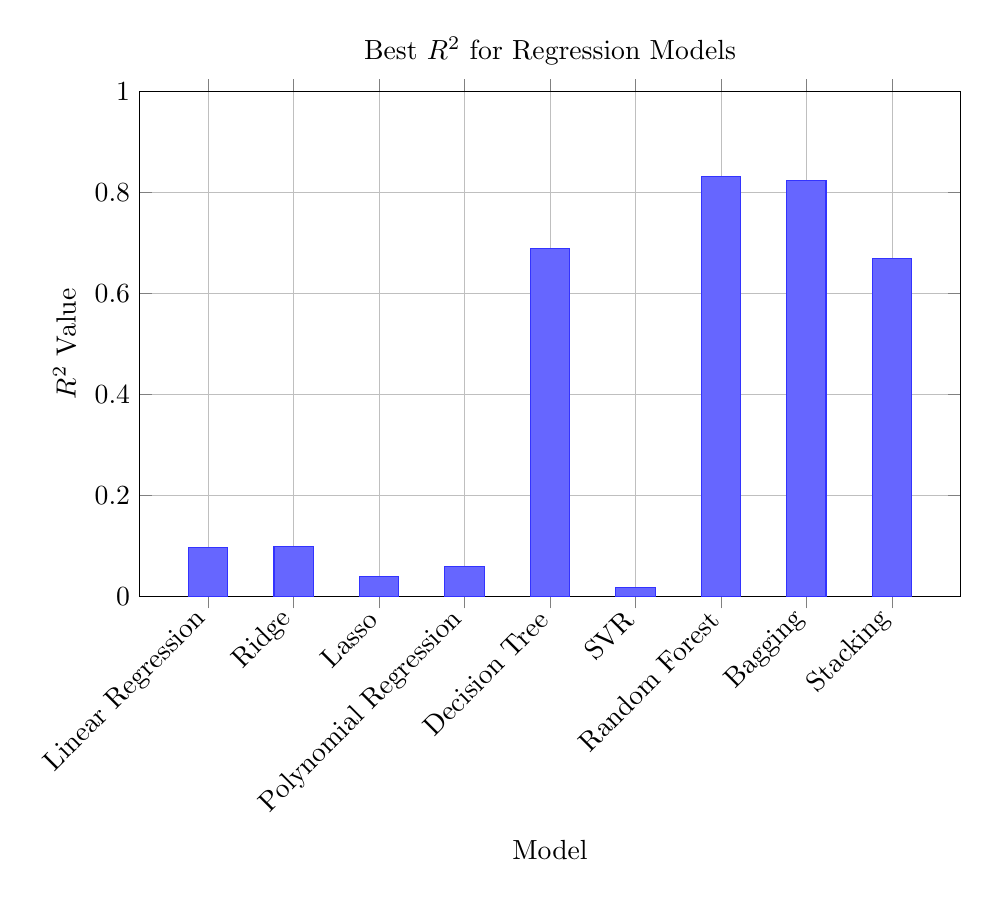
\begin{tikzpicture}
        \begin{axis}[
            ybar,
            width=12cm,
            height=8cm,
            bar width=0.5cm,
            xlabel={Model},
            ylabel={$R^2$ Value},
            title={Best $R^2$ for Regression Models},
            symbolic x coords={Linear Regression, Ridge, Lasso, Polynomial Regression, Decision Tree, SVR, Random Forest, Bagging, Stacking},
            xtick=data,
            xticklabel style={rotate=45, anchor=east},
            ymin=0, ymax=1,
            grid=major,
            major grid style={line width=0.2pt, gray!50},
        ]
        \addplot[fill=blue!60, draw=blue!80] coordinates {
            (Linear Regression, 0.0978)
            (Ridge, 0.0985)
            (Lasso, 0.0394)
            (Polynomial Regression, 0.0593)
            (Decision Tree, 0.6891)
            (SVR, 0.0183)
            (Random Forest, 0.8305)
            (Bagging, 0.8224)
            (Stacking, 0.6683)
        };
        \end{axis}
    \end{tikzpicture}
    \caption{Best $R^2$ for Regression Models}
    \label{fig:regression}
\end{figure}

\begin{enumerate}
    \item \textbf{最佳模型:}
    \begin{itemize}
        \item \texttt{Random Forest} 表现最好,最优 $R^2$ 值为 0.8305,解释了约 83.05\% 的目标变量方差,是所有模型中预测能力最强的。
        \item \texttt{Bagging} 紧随其后,$R^2$ 值为 0.8224,解释了 82.24\% 的方差,显示集成方法的稳健性。
        \item \texttt{Decision Tree} 表现良好,$R^2$ 值为 0.6891,解释了 68.91\% 的方差,优于线性模型,但逊于集成方法。
    \end{itemize}
    \item \textbf{线性模型表现:}
    \begin{itemize}
        \item \texttt{Ridge} ($R^2 = 0.0985$) 略优于 \texttt{Linear Regression} ($R^2 = 0.0978$),显示正则化带来轻微提升,但两者解释能力较弱,仅约 9.8\%。
        \item \texttt{Lasso} ($R^2 = 0.0394$) 表现极差,可能因强正则化剔除了过多特征,导致欠拟合。
    \end{itemize}
    \item \textbf{其他模型:}
    \begin{itemize}
        \item \texttt{多项式回归} ($R^2 = 0.0593$) 略优于 \texttt{Lasso},但远低于集成模型,表明二次特征帮助有限。
        \item \texttt{SVR} ($R^2 = 0.0183$) 表现最差,可能因核函数不适合该数据集或者正则化较弱。
        \item \texttt{Stacking} ($R^2 = 0.6683$) 性能一般,但未达随机森林和 \texttt{Bagging} 水平,模型组合或基模型选择需优化。
    \end{itemize}
    \item 集成方法(\texttt{Random Forest}和 \texttt{Bagging})显著优于其他模型,$R^2$ 值超 0.8,展现出较强的的非线性建模能力和鲁棒性。
    \item 线性模型(线性回归、Ridge、Lasso)和 SVR 表现不佳,$R^2$ 值低于 0.1,表明数据可能具复杂非线性关系,线性方法难以捕捉。
\end{enumerate}




\section{分类任务}

\subsection{模型以及指标选择}
\begin{itemize}
    \item 
    {
        在分类任务中,我主要探究了以下几种模型:
\begin{itemize}
    \item 线性模型:\texttt{Logistic Regression}
    \item 非线性模型:\texttt{Decision Tree}以及使用\texttt{'rbf'}核函数的\texttt{SVC}
    \item 集成学习:\texttt{Random Forest}、\texttt{Bagging}、\texttt{Voting}
\end{itemize}
    }
    \item 
    {
        在该任务中,我选用了\emph{Accuracy}、\emph{Weighted Precision}、\emph{Weighted Recall}、\emph{Weighted F1 score}以及\emph{Weighted OvR AUC}这几种指标。
\begin{itemize}
    \item \emph{Accuracy}: 
    \[
    \text{Accuracy} = \frac{\text{Number of Correct Predictions}}{\text{Total Number of Predictions}}
    \]

    \item \emph{Weighted Precision}:
    \[
    \text{Weighted Precision} = \sum_{i=1}^{N} w_i \cdot \text{Precision}_i
    \]
    其中,\(\text{Precision}_i = \frac{\text{TP}_i}{\text{TP}_i + \text{FP}_i}\),\(w_i = \frac{\text{Number of Samples in Class } i}{\text{Total Number of Samples}}\)。

    \item \emph{Weighted Recall}:
    \[
    \text{Weighted Recall} = \sum_{i=1}^{N} w_i \cdot \text{Recall}_i
    \]
    其中,\(\text{Recall}_i = \frac{\text{TP}_i}{\text{TP}_i + \text{FN}_i}\),\(w_i = \frac{\text{Number of Samples in Class } i}{\text{Total Number of Samples}}\)。

    \item \emph{Weighted F1 score}:
    \[
    \text{Weighted F1} = \sum_{i=1}^{N} w_i \cdot \text{F1}_i
    \]
    其中,\(\text{F1}_i = \frac{2 \cdot \text{Precision}_i \cdot \text{Recall}_i}{\text{Precision}_i + \text{Recall}_i}\)。

    \item \emph{Weighted OvR AUC}:
    \[
    \text{Weighted OvR AUC} = \sum_{i=1}^{N} w_i \cdot \text{AUC}_i
    \]
    其中,\(\text{AUC}_i\)表示对于类别 \(i\) 的 OvR(One-vs-Rest)模式下的曲线下面积,\(w_i = \frac{\text{Number of Samples in Class } i}{\text{Total Number of Samples}}\)。
\end{itemize}

    }
\end{itemize}

\subsection{线性模型}
\subsubsection{\texttt{Logistic Regression}}
在\texttt{Logistic Regression}中,我设置参数$C$的取值为$\left[0.01, 0.1, 1.0, 5\right]$,
并使用\texttt{GridSearchCV}来进行辅助参数搜索,得到以下结果。

\begin{table}[H]
    \centering
    \small % Reduce font size to fit content better
    \setlength{\tabcolsep}{3.5pt} % Adjust column padding for tighter fit
   \resizebox{\linewidth}{!}{
    \begin{tabular}{|l|c|c|c|c|c|c|c|c|c|c|}
    \hline
    \textbf{Feature Set} & \multicolumn{5}{c|}{\textbf{方法二}} & \multicolumn{5}{c|}{\textbf{方法三}} \\ \cline{2-11}
     & \textbf{Avg Acc} & \textbf{Avg Prec} & \textbf{Avg Rec} & \textbf{Avg F1} & \textbf{Avg AUC} & \textbf{Avg Acc} & \textbf{Avg Prec} & \textbf{Avg Rec} & \textbf{Avg F1} & \textbf{Avg AUC} \\ \hline
    Original & 0.7593 & 0.7538 & 0.7593 & 0.7015 & 0.5249 & 0.6896 & 0.6403 & 0.6896 & 0.5792 & 0.5623 \\ \hline
    PCA\_50 & 0.3309 & 0.6625 & 0.3309 & 0.3804 & 0.5933 & 0.5620 & 0.5856 & 0.5620 & 0.5642 & 0.5796 \\ \hline
    PCA\_100 & 0.3309 & 0.6625 & 0.3309 & 0.3804 & 0.5933 & 0.5620 & 0.5856 & 0.5620 & 0.5642 & 0.5796 \\ \hline
    PCA\_200 & 0.3309 & 0.6625 & 0.3309 & 0.3804 & 0.5933 & 0.5620 & 0.5857 & 0.5620 & 0.5642 & 0.5796 \\ \hline
    Select50Best & 0.7593 & 0.7538 & 0.7593 & 0.7015 & 0.5248 & 0.8593 & 0.8384 & 0.8593 & 0.8233 & 0.9238 \\ \hline
    Select100Best & 0.7593 & 0.7538 & 0.7593 & 0.7015 & 0.5249 & 0.6815 & 0.6268 & 0.6815 & 0.5982 & 0.4937 \\ \hline
    Select200Best & 0.7593 & 0.7538 & 0.7593 & 0.7015 & 0.5249 & 0.6896 & 0.6403 & 0.6896 & 0.5792 & 0.5623 \\ \hline
    LDA & 0.7718 & 0.7187 & 0.7718 & 0.7140 & 0.7248 & 0.8769 & 0.8682 & 0.8769 & 0.8692 & 0.9532 \\ \hline
    Scaled\_Original & 0.7718 & 0.7125 & 0.7718 & 0.7155 & 0.7092 & 0.8770 & 0.8686 & 0.8770 & 0.8701 & 0.9488 \\ \hline
    Scaled\_PCA\_50 & 0.7733 & 0.7389 & 0.7733 & 0.7139 & 0.7086 & 0.7904 & 0.7613 & 0.7904 & 0.7548 & 0.8431 \\ \hline
    Scaled\_PCA\_100 & 0.7733 & 0.7400 & 0.7733 & 0.7144 & 0.7093 & 0.8686 & 0.8561 & 0.8686 & 0.8528 & 0.9373 \\ \hline
    Scaled\_PCA\_200 & 0.7726 & 0.7172 & 0.7726 & 0.7145 & 0.7097 & 0.8731 & 0.8649 & 0.8731 & 0.8631 & 0.9454 \\ \hline
    Scaled\_Select50Best & 0.7522 & 0.7337 & 0.7522 & 0.7070 & 0.7063 & 0.8658 & 0.8408 & 0.8658 & 0.8389 & 0.9294 \\ \hline
    Scaled\_Select100Best & 0.7736 & 0.7390 & 0.7736 & 0.7146 & 0.7108 & 0.8746 & 0.8598 & 0.8746 & 0.8584 & 0.9393 \\ \hline
    Scaled\_Select200Best & 0.7720 & 0.7250 & 0.7720 & 0.7146 & 0.7096 & \textbf{0.8803} & 0.8714 & 0.8803 & 0.8725 & 0.9510 \\ \hline
    Scaled\_LDA & 0.7718 & 0.7187 & 0.7718 & 0.7140 & 0.7248 & 0.8768 & 0.8680 & 0.8768 & 0.8689 & 0.9531 \\ \hline
    \end{tabular}
    }
    \caption{Performance Metrics for Logistic Regression}
\end{table}

同样的,取出最优参数设置的模型,下面是每一折中的性能表现。
第一行子图为模型预测的混淆矩阵,第二行子图为模型的按类\texttt{ROC}曲线。

\begin{figure}[H]
    \centering
    \includegraphics[width=0.8\textwidth]{Figs/clf_Logistic_Regression.png}
    \caption{Logistic Regression}
\end{figure}

\begin{figure}[H]
    \centering
    \includegraphics[width=0.8\textwidth]{Figs/clf_Logistic_Regression_detailed.png}
    \caption{Logistic Regression}
\end{figure}

\subsection{非线性模型}
\subsubsection{\texttt{Decision Tree}}
在\texttt{Decision Tree}中,我设置树的最大深度取值为$\left[50, 100, 200\right]$,
并使用\texttt{GridSearchCV}进行参数搜索调优,得到下面的实验结果。

\begin{table}[H]
    \centering
    \small % Reduce font size to fit content better
    \setlength{\tabcolsep}{3.5pt} % Adjust column padding for tighter fit
   \resizebox{\linewidth}{!}{
    \begin{tabular}{|l|c|c|c|c|c|c|c|c|c|c|}
    \hline
    \textbf{Feature Set} & \multicolumn{5}{c|}{\textbf{方法二}} & \multicolumn{5}{c|}{\textbf{方法三}} \\ \cline{2-11}
     & \textbf{Avg Acc} & \textbf{Avg Prec} & \textbf{Avg Rec} & \textbf{Avg F1} & \textbf{Avg AUC} & \textbf{Avg Acc} & \textbf{Avg Prec} & \textbf{Avg Rec} & \textbf{Avg F1} & \textbf{Avg AUC} \\ \hline
    Original & 0.6421 & 0.6835 & 0.6421 & 0.6586 & 0.5972 & 0.8206 & 0.8254 & 0.8206 & 0.8227 & 0.8162 \\ \hline
    PCA\_50 & 0.6334 & 0.6739 & 0.6334 & 0.6505 & 0.5897 & 0.6601 & 0.6803 & 0.6601 & 0.6694 & 0.6663 \\ \hline
    PCA\_100 & 0.6299 & 0.6740 & 0.6299 & 0.6488 & 0.5859 & 0.6994 & 0.7156 & 0.6994 & 0.7069 & 0.7011 \\ \hline
    PCA\_200 & 0.6219 & 0.6681 & 0.6219 & 0.6411 & 0.5813 & 0.7229 & 0.7311 & 0.7229 & 0.7267 & 0.6829 \\ \hline
    Select50Best & 0.6461 & 0.6915 & 0.6461 & 0.6652 & 0.6089 & 0.8030 & 0.8183 & 0.8030 & 0.8100 & 0.8094 \\ \hline
    Select100Best & 0.6494 & 0.6883 & 0.6494 & 0.6660 & 0.6068 & 0.8128 & 0.8220 & 0.8128 & 0.8170 & 0.8110 \\ \hline
    Select200Best & 0.6405 & 0.6829 & 0.6405 & 0.6576 & 0.5968 & 0.8253 & 0.8308 & 0.8253 & 0.8277 & 0.8222 \\ \hline
    LDA & 0.6181 & 0.6567 & 0.6181 & 0.6352 & 0.5688 & \textbf{0.8296} & 0.8315 & 0.8296 & 0.8305 & 0.8260 \\ \hline
    Scaled\_Original & 0.6449 & 0.6843 & 0.6449 & 0.6609 & 0.5993 & 0.8176 & 0.8249 & 0.8176 & 0.8208 & 0.8145 \\ \hline
    Scaled\_PCA\_50 & 0.6321 & 0.6741 & 0.6321 & 0.6500 & 0.5891 & 0.6612 & 0.6815 & 0.6612 & 0.6706 & 0.6674 \\ \hline
    Scaled\_PCA\_100 & 0.6260 & 0.6728 & 0.6260 & 0.6459 & 0.5849 & 0.6991 & 0.7158 & 0.6991 & 0.7068 & 0.6979 \\ \hline
    Scaled\_PCA\_200 & 0.6240 & 0.6680 & 0.6240 & 0.6422 & 0.5808 & 0.7242 & 0.7328 & 0.7242 & 0.7282 & 0.6942 \\ \hline
    Scaled\_Select50Best & 0.6453 & 0.6902 & 0.6453 & 0.6642 & 0.6069 & 0.8033 & 0.8178 & 0.8033 & 0.8100 & 0.8090 \\ \hline
    Scaled\_Select100Best & 0.6477 & 0.6890 & 0.6477 & 0.6651 & 0.6063 & 0.8134 & 0.8235 & 0.8134 & 0.8179 & 0.8124 \\ \hline
    Scaled\_Select200Best & 0.6418 & 0.6839 & 0.6418 & 0.6586 & 0.5973 & 0.8248 & 0.8309 & 0.8248 & 0.8275 & 0.8210 \\ \hline
    Scaled\_LDA & 0.6203 & 0.6581 & 0.6203 & 0.6372 & 0.5702 & 0.8289 & 0.8311 & 0.8289 & 0.8299 & 0.8250 \\ \hline
    \end{tabular}
    }
    \caption{Performance Metrics for Decision Tree}
\end{table}

同样的,取出最优参数设置的模型,下面是每一折中的性能表现。

\begin{figure}[H]
    \centering
    \includegraphics[width=0.8\textwidth]{Figs/clf_Deision_Tree.png}
    \caption{Decision Tree}
\end{figure}

\begin{figure}[H]
    \centering
    \includegraphics[width=0.8\textwidth]{Figs/clf_Decision_Tree_detailed.png}
    \caption{Decision Tree}
\end{figure}

\subsubsection{\texttt{SVC}}
在\texttt{SVC}中,由于算力资源有限,我无法进行参数搜索,
同时设置较低的正则化力度,选用较简单的非线性核函数。
故设置$C=0.1$,核函数选择\texttt{'rbf'},
只进行了六组简单的实验,结果如下。

\begin{table}[H]
    \centering
    \small % Reduce font size to fit content better
    \setlength{\tabcolsep}{3.5pt} % Adjust column padding for tighter fit
   \resizebox{\linewidth}{!}{
    \begin{tabular}{|l|c|c|c|c|c|c|c|c|c|c|}
    \hline
    \textbf{Feature Set} & \multicolumn{5}{c|}{\textbf{方法二}} & \multicolumn{5}{c|}{\textbf{方法三}} \\ \cline{2-11}
     & \textbf{Avg Acc} & \textbf{Avg Prec} & \textbf{Avg Rec} & \textbf{Avg F1} & \textbf{Avg AUC} & \textbf{Avg Acc} & \textbf{Avg Prec} & \textbf{Avg Rec} & \textbf{Avg F1} & \textbf{Avg AUC} \\ \hline
    Scaled\_PCA\_50 & 0.7666 & 0.7703 & 0.7666 & 0.6876 & 0.7085 & 0.7834 & 0.8035 & 0.7834 & 0.7327 & 0.8417 \\ \hline
    Scaled\_Select50Best & 0.7669 & 0.7722 & 0.7669 & 0.6881 & 0.7025 & 0.8563 & 0.8649 & 0.8563 & 0.8175 & 0.9196 \\ \hline
    Scaled\_LDA & 0.7732 & 0.7742 & 0.7732 & 0.7123 & 0.6449 & \textbf{0.8782} & 0.8693 & 0.8782 & 0.8678 & 0.9201 \\ \hline
    \end{tabular}
    }
    \caption{Performance Metrics for SVC}
\end{table}

同样的,取出最优参数设置的模型,下面是每一折中的性能表现。

\begin{figure}[H]
    \centering
    \includegraphics[width=0.8\textwidth]{Figs/clf_SVC.png}
    \caption{SVC}
\end{figure}

\begin{figure}[H]
    \centering
    \includegraphics[width=0.8\textwidth]{Figs/clf_SVC_detailed.png}
    \caption{SVC}
\end{figure}


\subsection{集成算法}
\subsubsection{\texttt{Random Forest}}
在\texttt{Random Forest}中,我设置树的数量分别为$\left[50, 100\right]$,
最大深度分别为$\left[100, 200\right]$,然后使用\texttt{GridSearchCV}进行辅助参数调优。
同样由于算力资源有限,我只进行了下面较为简单的十六组实验。

\begin{table}[H]
    \centering
    \small % Reduce font size to fit content better
    \setlength{\tabcolsep}{3.5pt} % Adjust column padding for tighter fit
   \resizebox{\linewidth}{!}{
    \begin{tabular}{|l|c|c|c|c|c|c|c|c|c|c|}
    \hline
    \textbf{Feature Set} & \multicolumn{5}{c|}{\textbf{方法二}} & \multicolumn{5}{c|}{\textbf{方法三}} \\ \cline{2-11}
     & \textbf{Avg Acc} & \textbf{Avg Prec} & \textbf{Avg Rec} & \textbf{Avg F1} & \textbf{Avg AUC} & \textbf{Avg Acc} & \textbf{Avg Prec} & \textbf{Avg Rec} & \textbf{Avg F1} & \textbf{Avg AUC} \\ \hline
    Original & 0.7802 & 0.7300 & 0.7802 & 0.7240 & 0.7254 & \textbf{0.8840} & 0.8828 & 0.8840 & 0.8659 & 0.9587 \\ \hline
    PCA\_50 & 0.7793 & 0.7362 & 0.7793 & 0.7242 & 0.7184 & 0.7989 & 0.7880 & 0.7989 & 0.7569 & 0.8559 \\ \hline
    Select50Best & 0.7782 & 0.7343 & 0.7782 & 0.7332 & 0.7442 & 0.8817 & 0.8651 & 0.8817 & 0.8616 & 0.9386 \\ \hline
    LDA & 0.7573 & 0.6989 & 0.7573 & 0.7148 & 0.6824 & 0.8793 & 0.8705 & 0.8793 & 0.8724 & 0.9471 \\ \hline
    Scaled\_Original & 0.7796 & 0.7280 & 0.7796 & 0.7230 & 0.7279 & 0.8834 & 0.8827 & 0.8834 & 0.8647 & 0.9590 \\ \hline
    Scaled\_PCA\_50 & 0.7781 & 0.7500 & 0.7781 & 0.7231 & 0.7173 & 0.7990 & 0.7974 & 0.7990 & 0.7570 & 0.8547 \\ \hline
    Scaled\_Select50Best & 0.7781 & 0.7323 & 0.7781 & 0.7330 & 0.7431 & 0.8820 & 0.8651 & 0.8820 & 0.8616 & 0.9392 \\ \hline
    Scaled\_LDA & 0.7571 & 0.6988 & 0.7571 & 0.7148 & 0.6819 & 0.8792 & 0.8700 & 0.8792 & 0.8723 & 0.9465 \\ \hline
    \end{tabular}
    }
    \caption{Performance Metrics for Random Forest}
\end{table}

同样的,取出最优参数设置的模型,下面是每一折中的性能表现。

\begin{figure}[H]
    \centering
    \includegraphics[width=0.8\textwidth]{Figs/clf_Random_Forest.png}
    \caption{Random Forest}
\end{figure}

\begin{figure}[H]
    \centering
    \includegraphics[width=0.8\textwidth]{Figs/clf_Random_Forest_detailed.png}
    \caption{Random Forest}
\end{figure}

\subsubsection{\texttt{Bagging}}

在\texttt{Bagging}中,\texttt{estimator}我选择了最大深度为$C=0.1$的\texttt{Logistic Regression},
并设置\texttt{estimator}数量为10,进行了下面的实验。

\begin{table}[H]
    \centering
    \small % Reduce font size to fit content better
    \setlength{\tabcolsep}{3.5pt} % Adjust column padding for tighter fit
   \resizebox{\linewidth}{!}{
    \begin{tabular}{|l|c|c|c|c|c|c|c|c|c|c|}
    \hline
    \textbf{Feature Set} & \multicolumn{5}{c|}{\textbf{Method 2}} & \multicolumn{5}{c|}{\textbf{Method 3}} \\ \cline{2-11}
     & \textbf{Avg Acc} & \textbf{Avg Prec} & \textbf{Avg Rec} & \textbf{Avg F1} & \textbf{Avg AUC} & \textbf{Avg Acc} & \textbf{Avg Prec} & \textbf{Avg Rec} & \textbf{Avg F1} & \textbf{Avg AUC} \\ \hline
    Original & 0.7595 & 0.7540 & 0.7595 & 0.7016 & 0.5255 & 0.6898 & 0.6123 & 0.6898 & 0.5858 & 0.6023 \\ \hline
    PCA\_50 & 0.3331 & 0.6619 & 0.3331 & 0.3805 & 0.5929 & 0.5787 & 0.5932 & 0.5787 & 0.5797 & 0.5846 \\ \hline
    PCA\_100 & 0.3332 & 0.6618 & 0.3332 & 0.3807 & 0.5929 & 0.5787 & 0.5932 & 0.5787 & 0.5797 & 0.5847 \\ \hline
    PCA\_200 & 0.3333 & 0.6619 & 0.3333 & 0.3807 & 0.5929 & 0.5783 & 0.5931 & 0.5783 & 0.5795 & 0.5847 \\ \hline
    Select50Best & 0.7595 & 0.7539 & 0.7595 & 0.7014 & 0.5253 & 0.8594 & 0.8365 & 0.8594 & 0.8237 & 0.9236 \\ \hline
    Select100Best & 0.7594 & 0.7539 & 0.7594 & 0.7015 & 0.5253 & 0.6991 & 0.5953 & 0.6991 & 0.5830 & 0.4475 \\ \hline
    Select200Best & 0.7594 & 0.7538 & 0.7594 & 0.7013 & 0.5253 & 0.6900 & 0.6119 & 0.6900 & 0.5857 & 0.6024 \\ \hline
    LDA & 0.7718 & 0.7218 & 0.7718 & 0.7143 & 0.7249 & 0.8767 & 0.8680 & 0.8767 & 0.8690 & 0.9532 \\ \hline
    Scaled\_Original & 0.7722 & 0.7171 & 0.7722 & 0.7176 & 0.7098 & 0.8769 & 0.8678 & 0.8769 & 0.8697 & 0.9484 \\ \hline
    Scaled\_PCA\_50 & 0.7730 & 0.7381 & 0.7730 & 0.7140 & 0.7089 & 0.7915 & 0.7610 & 0.7915 & 0.7567 & 0.8467 \\ \hline
    Scaled\_PCA\_100 & 0.7726 & 0.7376 & 0.7726 & 0.7148 & 0.7095 & 0.8687 & 0.8565 & 0.8687 & 0.8546 & 0.9372 \\ \hline
    Scaled\_PCA\_200 & 0.7622 & 0.7170 & 0.7622 & 0.7167 & 0.7048 & 0.8713 & 0.8633 & 0.8713 & 0.8626 & 0.9446 \\ \hline
    Scaled\_Select50Best & 0.7738 & 0.7414 & 0.7738 & 0.7159 & 0.7132 & 0.8655 & 0.8412 & 0.8655 & 0.8387 & 0.9293 \\ \hline
    Scaled\_Select100Best & 0.7733 & 0.7406 & 0.7733 & 0.7158 & 0.7114 & 0.8747 & 0.8603 & 0.8747 & 0.8595 & 0.9392 \\ \hline
    Scaled\_Select200Best & 0.7726 & 0.7232 & 0.7726 & 0.7165 & 0.7107 & \textbf{0.8793} & 0.8703 & 0.8793 & 0.8718 & 0.9500 \\ \hline
    Scaled\_LDA & 0.7718 & 0.7218 & 0.7718 & 0.7143 & 0.7249 & 0.8767 & 0.8681 & 0.8767 & 0.8690 & 0.9532 \\ \hline
    \end{tabular}
    }
    \caption{Performance Metrics for Bagging}
\end{table}

同样的,取出最优参数设置的模型,下面是每一折中的性能表现。

\begin{figure}[H]
    \centering
    \includegraphics[width=0.8\textwidth]{Figs/clf_Bagging.png}
    \caption{Bagging}
\end{figure}

\begin{figure}[H]
    \centering
    \includegraphics[width=0.8\textwidth]{Figs/clf_Bagging_detailed.png}
    \caption{Bagging}
\end{figure}

\subsubsection{\texttt{Voting}}
在\texttt{Voting}中,我使用了三个\texttt{estimator}:
\begin{itemize}
    \item 最大深度为200的\texttt{Decision Tree}
    \item 使用默认参数的\texttt{SVC}
    \item $C=0.5$的\texttt{Logistic Regression}
\end{itemize}
并使用\textbf{软投票}的策略。由于算力资源有限,我只做了下面六组简单的实验。

\begin{table}[H]
    \centering
    \small % Reduce font size to fit content better
    \setlength{\tabcolsep}{3.5pt} % Adjust column padding for tighter fit
    \resizebox{\linewidth}{!}{
    \begin{tabular}{|l|c|c|c|c|c|c|c|c|c|c|}
    \hline
    \textbf{Feature Set} & \multicolumn{5}{c|}{\textbf{Method 2}} & \multicolumn{5}{c|}{\textbf{Method 3}} \\ \cline{2-11}
     & \textbf{Avg Acc} & \textbf{Avg Prec} & \textbf{Avg Rec} & \textbf{Avg F1} & \textbf{Avg AUC} & \textbf{Avg Acc} & \textbf{Avg Prec} & \textbf{Avg Rec} & \textbf{Avg F1} & \textbf{Avg AUC} \\ \hline
    Scaled\_PCA\_50 & 0.7620 & 0.7075 & 0.7620 & 0.7232 & 0.6998 & 0.7788 & 0.7414 & 0.7788 & 0.7526 & 0.8366 \\ \hline
    Scaled\_Select50Best & 0.7629 & 0.7138 & 0.7629 & 0.7270 & 0.7075 & 0.8692 & 0.8484 & 0.8692 & 0.8520 & 0.9348 \\ \hline
    Scaled\_LDA & 0.7601 & 0.6978 & 0.7601 & 0.7148 & 0.6907 & \textbf{0.8802} & 0.8700 & 0.8802 & 0.8710 & 0.9492 \\ \hline
    \end{tabular}
    }
    \caption{Performance Metrics for Voting}
\end{table}

同样的,取出最优参数设置的模型,下面是每一折中的性能表现。

\begin{figure}[H]
    \centering
    \includegraphics[width=0.8\textwidth]{Figs/clf_Voting.png}
    \caption{Voting}
\end{figure}

\begin{figure}[H]
    \centering
    \includegraphics[width=0.8\textwidth]{Figs/clf_Voting_detailed.png}
    \caption{Voting}
\end{figure}

\subsection{分类任务小结}
\subsubsection{一些观察与思考}
\begin{itemize}
    \item 通过混淆矩阵不难看出,类别1的占比是很大的,这导致我们在衡量模型性能的时候
    朴素地取各个指标关于类别的平均值是不太合理的。因此,在衡量模型的性能的时候,
    对各个指标进行关于类别占比的加权是有必要的。
\end{itemize}

\subsubsection{模型性能比较}
\begin{figure}[h]
    \centering
    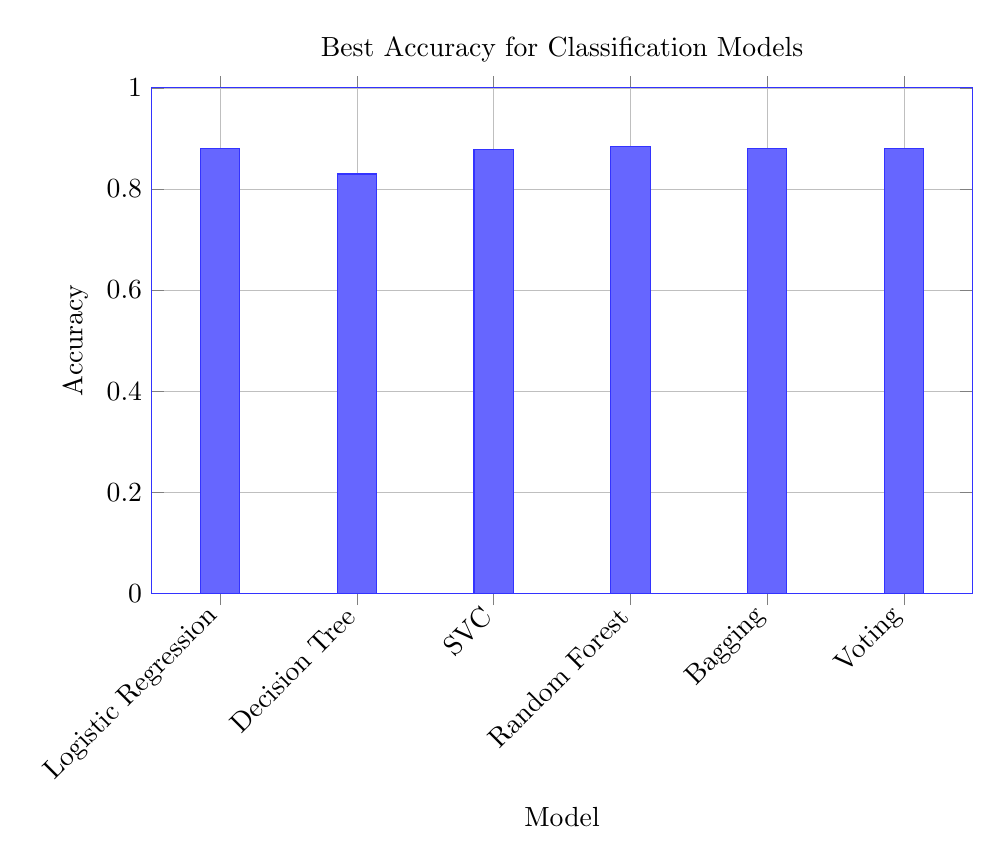
\begin{tikzpicture}
        \begin{axis}[
            ybar,
            width=12cm,
            height=8cm,
            bar width=0.5cm,
            xlabel={Model},
            ylabel={Accuracy},
            title={Best Accuracy for Classification Models},
            symbolic x coords={Logistic Regression, Decision Tree, SVC, Random Forest, Bagging, Voting},
            xtick=data,
            xticklabel style={rotate=45, anchor=east},
            ymin=0, ymax=1,
            grid=major,
            major grid style={line width=0.2pt, gray!50},
            fill=blue!60,
            draw=blue!80
        ]
        \addplot[fill=blue!60, draw=blue!80] coordinates {
            (Logistic Regression, 0.8803)
            (Decision Tree, 0.8296)
            (SVC, 0.8782)
            (Random Forest, 0.8840)
            (Bagging, 0.8793)
            (Voting, 0.8802)
        };
        \end{axis}
    \end{tikzpicture}  
    \caption{Best Accuracy for Classification Models}
    \label{fig:classification}
\end{figure}

\begin{enumerate}
    \item \textbf{最佳模型:}
    \begin{itemize}
        \item \texttt{Random Forest} 性能表现最好,最优准确率为 0.8840。
        \item \texttt{Logistic Regression} (准确率 = 0.8803) 和 \texttt{Voting} (准确率 = 0.8802) 表现相近,均接近 88\%,显示稳健性能。
        \item \texttt{Bagging} (准确率 = 0.8793) 和 \texttt{SVC} (准确率 = 0.8782) 表现良好,准确率超 87.8\%,接近最佳模型。
    \end{itemize}
    \item \textbf{其他模型:}
    \begin{itemize}
        \item \texttt{Decision Tree} (准确率 = 0.8296) 表现最弱,但仍正确分类 82.96\% 的样本,可能因过拟合或树深度设置不当。
    \end{itemize}
    \item \textbf{模型比较:}
    \begin{itemize}
        \item 集成方法(\texttt{Random Forest}、\texttt{Bagging}、\texttt{Voting})表现优异,准确率超 0.87,表明结合多模型或抽样策略有效提升分类性能。
        \item \texttt{Logistic Regression} 作为线性模型,准确率达 0.8803,接近集成方法,表明数据可能适合线性分离。
        \item \texttt{SVC} 表现稳健,准确率为 0.8782,说明非线性核函数对任务有效。
    \end{itemize}
\end{enumerate}

\section{总结}
\begin{itemize}
    \item 在较简单的模型(如线性模型以及\texttt{Polynomial Regression}中,
    使用方法二和方法三处理数据最终的性能并没有明显的差距,但是在更复杂模型中,
    普遍方法三的性能要优于方法二,我的猜测是由于方法二处理过后的数据方差较小,
    并且丢失了一些特征,导致复杂模型能学到的“知识”不足,进而导致欠拟合。
    \item 综合上述模型,发现同目标维度相同的特征选择的性能要普遍优于主成分分析,
    我猜想这可能是由于特征选择中存在一个辅助评分函数,能使降维得到的数据更能表征数据。
    \item 关于降维的目标维度,从上述结果不难看出,对于较简单的模型,随着目标维度的上升,
    性能普遍会下降,这可能是由于模型过于简单,对于较复杂的数据的处理能力较弱。
    反观如\texttt{Random Forest}、\texttt{Bagging}等较为复杂的模型,
    在数据维度较高的情况下表现会比低维情况好,这可能是因为较低维度的数据会导致模型欠拟合。
    \item 关于数据归一化影响,在较简单的模型中,归一化后的表现普遍较未归一化的表现要好,
    但在较为复杂的模型中,是否进行归一化的影响没有那么强,这也体现出了复杂的模型对数据有更好的鲁棒性。
    \item 在使用集成算法时,estimator的数量很关键,使用了更多的estimator,
    会使模型更趋于复杂,也能有更好的鲁棒性,如\texttt{Bagging}和\texttt{Voting}
    使用的estimator数量较\texttt{Random Forest}少,会趋于在较低维度的数据上表现好,
    但使用较多的estimator的代价是算力资源消耗较多。
    通过特征学习技术,模型能在较低集成规模的情况下也能有不错的性能表现。
\end{itemize}

\end{document}